\section{Les particules du modèle standard}\label{chapter-MS-MSSM-section-SM_ptcs}
Une particule est considérée comme fondamentale si elle ne possède pas de sous-structure observée à ce jour. %ptc fondamentale = ? 10e-18 m
Le modèle standard décrit le comportement de ces particules fondamentales qui peuvent être catégorisées selon plusieurs critères.
Le premier d'entre eux est le \og spin \fg, une observable quantique intrinsèque aux particules.
Les particules de spin demi-entier sont les fermions, celles de spin entier les bosons.
\begin{figure}[h]
\centering
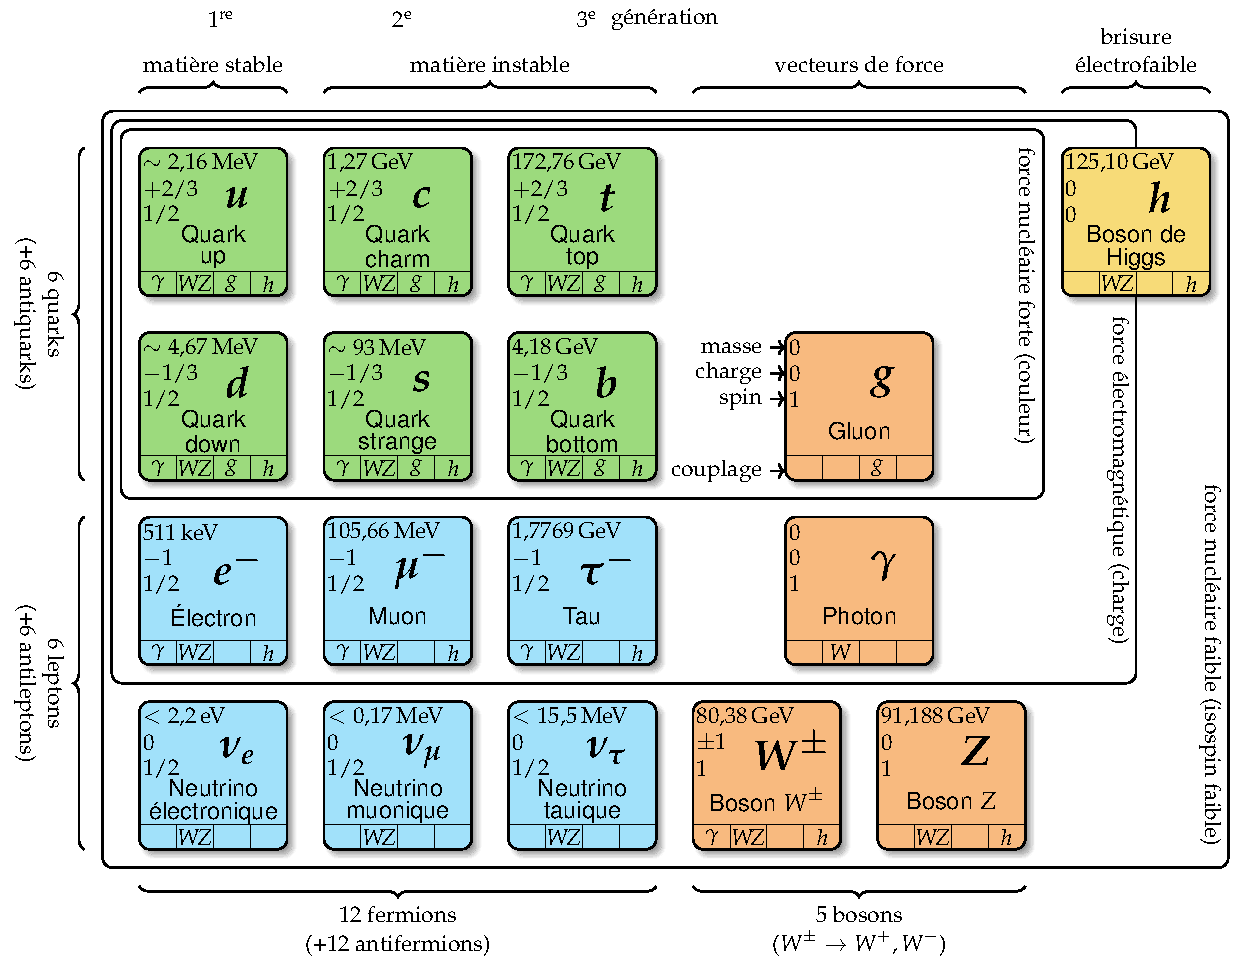
\includegraphics[width=\textwidth]{\PhDthesisdir/plots_and_images/Particles_tables/SM2018_FR.pdf}
\caption{Les particules fondamentales du modèle standard.}
\label{fig-MS-table}
\end{figure}

\subsection{Les fermions}\label{chapter-MS-MSSM-section-SM_ptcs-subsec-fermions}
Les fermions sont les particules fondamentales de spin demi-entier et suivent donc la statistique de Fermi-Dirac.
Ainsi, deux fermions ne peuvent pas occuper le même état quantique, \ie\ avoir chacun de leurs nombres quantiques égaux entre eux, comme exposé par le principe d'exclusion de Pauli.
Le modèle standard comprend douze fermions constituant la matière, accompagnés de douze antifermions correspondants pour l'antimatière.
\par Les fermions peuvent se diviser d'une part en deux catégories, les quarks et les leptons, et d'autre part en trois catégories correspondant à trois \og générations \fg, comme illustré sur la figure~\ref{fig-MS-table}. La première génération (quarks~\quarku\ et~\quarkd, électron \electron\ et neutrino électronique \nuele) correspond aux particules les plus communes; les deuxièmes et troisièmes générations contiennent des particules analogues, plus massives et instables.
% générations supplémentaires et boson Z ?
% spin demi entier (stat Fermi-Dirac -> exclusion Pauli (expliquer) et relation anticommutation). Constituants de la matière, il y en a 12.

\subsubsection{Les quarks}\label{chapter-MS-MSSM-section-SM_ptcs-subsec-fermions-subsubsec-quarks}
Les quarks sont les fermions possédant une charge de couleur.
Il existe deux quarks par génération, un quark de type \emph{up} et un quark de type \emph{down}, formant un doublet d'isospin faible.
L'isospin faible est un nombre quantique décrit dans la section~\ref{chapter-MS-MSSM-section-formalisme-subsec-EW}.
Il y a donc six quarks au total. Les quarks de type \emph{up} (\quarku, \quarkc\ et~\quarkt) portent une charge électrique $+\frac{2}{3}e$ avec $e$ la charge électrique élémentaire, les quarks de type \emph{down} (\quarkd, \quarks\ et~\quarkb) une charge $-\frac{1}{3}e$. Les antiquarks possèdent une charge électrique opposée ($-\frac{2}{3}e$ et $+\frac{1}{3}e$). Les quarks sont donc sensibles à l'interaction électromagnétique.
\par À l'instar de la charge électrique pour l'interaction électromagnétique, la \og couleur \fg rend les quarks sensibles à l'interaction forte. La charge de couleur peut prendre trois valeurs orthogonales, nommées par convention rouge, verte et bleue, car les particules portant une charge de couleur ne sont pas stables à elles seules et se regroupent pour former des particules composites de charge de couleur nulle, ou de couleur \og blanche \fg. C'est ce que l'on appelle le phénomène de \og confinement de couleur \fg, décrit dans la section~\ref{chapter-MS-MSSM-section-formalisme-subsec-QCD-subsubsec-confinement}.
\par Les particules composées de quarks sont les hadrons. Ces particules sont de couleur blanche, ce qui peut être obtenu de deux manières:
\begin{itemize}
\item par association d'un quark rouge, un vert et un bleu; il s'agit d'un \og baryon \fg. Le proton (\quarku\quarku\quarkd) et le neutron (\quarku\quarkd\quarkd) sont deux exemples de baryons.
\item par association d'un quark et d'un antiquark; il s'agit d'un \og méson \fg. En effet, un antiquark porte une \og anticouleur \fg. Ainsi, un quark up (\quarku) rouge et un antiquark down (\antiquarkd) \og antirouge \fg{} forment un pion chargé \pionplus.
\end{itemize}
\par Enfin, comme tous les fermions, les quarks sont également sensibles à l'interaction faible. Les quarks sont ainsi les seules particules sensibles à toutes les interactions fondamentales décrites par le modèle standard.
% fermions avec couleur = charge de la force forte, il y a en trois (orthogonales) + anticouleur. RGB. Weak isopsin doublet, trois doublets, 6 quarks. noms, charges.
%confinement, see other section. Particules de couleur \og blanche \fg{}. Hadrons. Mesons, Baryons. Protons et neutrons dans la matière.

\subsubsection{Les leptons}\label{chapter-MS-MSSM-section-SM_ptcs-subsec-fermions-subsubsec-leptons}
Les leptons sont les fermions ne possédant pas de charge de couleur. Ils sont donc insensibles à l'interaction forte. En revanche, ils sont tous sensibles à l'interaction faible.
Sur le même principe que pour les quarks, il y a un doublet d'isospin faible de deux leptons par génération, soit six leptons au total.
Les leptons d'isospin faible haut sont l'électron (\electron), le muon (\muon) et le tau (\leptau), ils portent une charge électrique $-e$ ($+e$ pour les antiparticules correspondantes). Les leptons d'isospin faible bas sont les neutrinos. Les neutrinos ne portent pas de charge électrique et interagissent donc uniquement par interaction faible, ce qui en fait des particules difficiles à détecter.
% pas de couleur, insensibles interaction forte. trois générations, weak isospin doublet. electron-like + neutrino $\times3=6$ leptons. charges électriques. Neutrinos, faible masse. Uniquement force faible, \emph{elusive particles}. Difficile à détecter.


\subsection{Les bosons}\label{chapter-MS-MSSM-section-SM_ptcs-subsec-bosons}
Les bosons sont les particules fondamentales de spin entier.
Ils suivent la statistique de Bose-Einstein qui n'interdit pas la présence de plusieurs bosons ayant tous leurs nombres quantiques égaux entre eux, contrairement à la statistique de Fermi-Dirac.
\par Les bosons de spin 1 sont les bosons de jauge, ou bosons vecteurs, et sont les médiateurs des interaction fondamentales.
Ainsi, le photon (\photon) est le boson vecteur de l'interaction électromagnétique. Il est de masse nulle et est électriquement neutre.
Les bosons \Wbosonplus, \Wbosonminus\ et \Zboson\ sont ceux de l'interaction faible. Le boson \Zboson\ est électriquement neutre et de masse $m_\Zboson=\SI{91.19}{\GeV}$, les bosons \Wboson\ portent une charge électrique de $\pm e$, ont une masse de $m_\Wboson=\SI{80.38}{\GeV}$ et n'interagissent qu'avec les particules de chiralité gauche et les antiparticules de chiralité droite.
La chiralité est définie dans la section~\ref{chapter-MS-MSSM-section-formalisme-subsec-EW}.
Enfin, huit gluons (\gluon) sont les médiateurs de l'interaction forte. Ils n'ont ni masse ni charge électrique, mais portent une charge de couleur et une charge d'anticouleur. Un gluon peut donc être chargé \og rouge et antibleu \fg{}. Si un tel gluon interagit avec un quark bleu, par conservation, ce quark est rouge après interaction.
\par Le boson de Higgs est de spin nul, il s'agit donc d'un boson scalaire. Ce boson est une conséquence du mécanisme de brisure spontanée de symétrie électrofaible, mécanisme donnant leurs masses aux particules. Ce mécanisme est présenté dans la section~\ref{chapter-MS-MSSM-section-formalisme-subsec-Higgs_mechanism}.

%spin entier, 1 (bosons de jauge, bosons vecteurs, vecteurs de force) ou 0 (Higgs). Bosons de jauge = vecteurs des forces fondamentales. Lesquels pour lesquelles.
%\Wboson\ et ptcs chiralité gauche antiptcs droite.
%8 gluons (pourquoi)
%
%\Wboson\ et chiralité?
%
%Higgs : up-to-date mass + bib ref
